\documentclass[border=4pt]{standalone}
\usepackage{tikz}
\usetikzlibrary{arrows.meta,fit,positioning}

\begin{document}
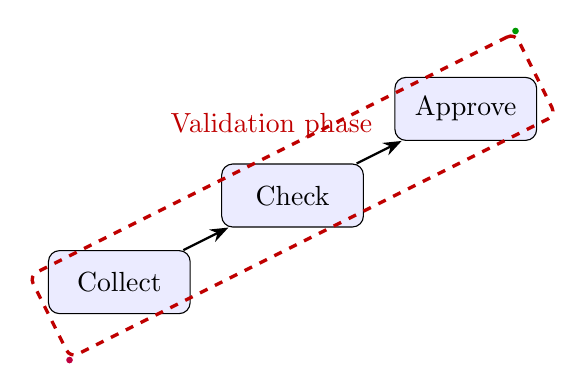
\begin{tikzpicture}[
  >=Stealth,
  process/.style={draw,rounded corners,minimum width=18mm,minimum height=8mm,fill=blue!8},
  flow/.style={->,thick}
]
  \node[process] (collect) at (0,0) {Collect};
  \node[process] (check) at (2.2,1.1) {Check};
  \node[process] (approve) at (4.4,2.2) {Approve};
  \draw[flow] (collect) -- (check);
  \draw[flow] (check) -- (approve);

  \node[rotate fit=26.565,fit=(collect)(check)(approve),
    draw=red!75!black,dashed,line width=1.2pt,rounded corners=3pt,inner sep=5pt] (phase) {};
  \node[above=2pt,text=red!75!black] at (phase.north) {Validation phase};
  \fill[green!60!black] (phase.north east) circle (1.2pt);
  \fill[purple] (phase.south west) circle (1.2pt);
\end{tikzpicture}
\end{document}
